\chapter{基于分布式文件系统GlusterFS的数据迁移研究}

\section{GlusterFS介绍}

\subsection{GlusterFS整体架构和原理}


GlusterFS\cite{GlusterFS}是一个开源、扩展能力强大的分布式文件系统,目前被广泛应用于各类商业存储服务器集群,其主要特性如下:
\begin{itemize}
    \item 全局命名空间。
    \item 集群存储管理。
    \item 模块化的层次机构。
    \item 内置replication and geo-replication特性。
    \item 自修复功能。
    \item 高效负载均衡。
\end{itemize}
\begin{figure}[htp]
\centering
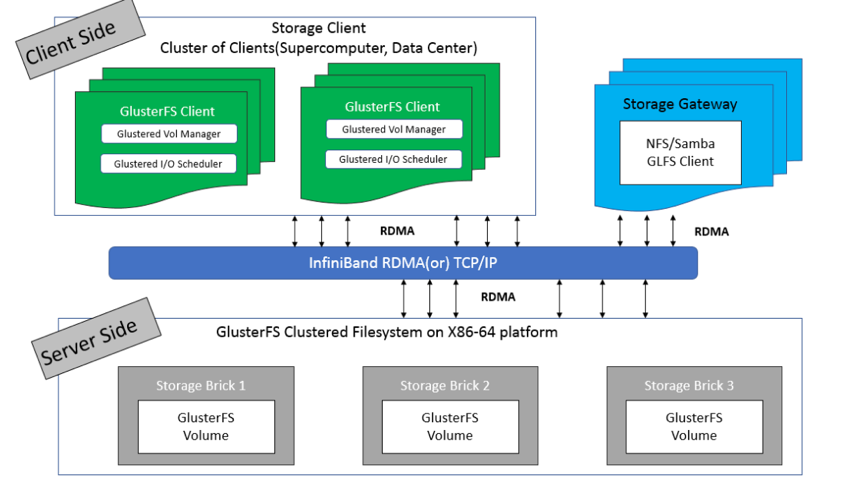
\includegraphics[width=\textwidth]{GlusterFS_Arc}
\caption{GlusterFS整体架构图}
\label{fig:GlusterFS_Arc}
\end{figure}
如图\ref{fig:GlusterFS_Arc}所示,GlusterFS的客户端与存储服务器可通过InfiniBand RDMA或者TCP/IP等多种方式连接,具有可扩展性、高性能、高可用性等特点。
\begin{itemize}
    \item 可扩展性:GlusterFS服务端以存储块(Storage Brick)为硬件存储单元,可挂载于磁盘、固态硬盘、内存等多种存储介质。逻辑卷(Volume)是文件系统中的逻辑存储单元,每一个逻辑卷可由一个或者多个存储块构成。
    \item 高性能:
    \item 高可用性:
\end{itemize}
GlusterFS的用户空间采用堆栈式设计,

\begin{figure}[htp]
\centering
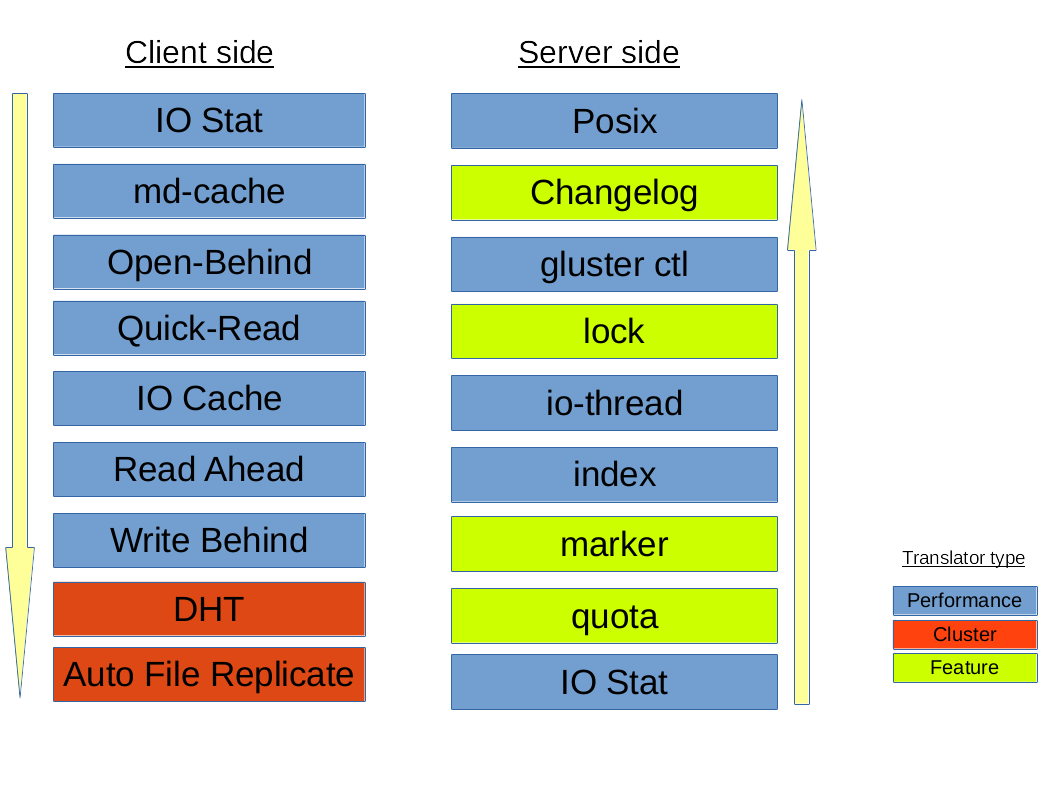
\includegraphics[width=\textwidth]{translators}
\caption{由翻译器(Translators)堆叠组成的堆栈式结构}
\label{fig:translators}
\end{figure}
\section{基于GlusterFS Tiering功能的缓存管理模块设计}
\subsection{Trace 模块}
\subsection{访问模式识别模型建立}
\subsection{运行时缓存管理}


\section{本章小结}